\documentclass{article}
\usepackage[utf8]{inputenc}

\title{Homework 1 PGM}
\author{Sharone Dayan, Michael Sutton }
\date{October 2017}
\usepackage[utf8]{inputenc}
\usepackage[french]{babel}
\usepackage{natbib}
\usepackage{graphicx}
\usepackage{enumitem}
\usepackage{mathtools}
\usepackage{amsmath}
\usepackage{dsfont}
\usepackage{stmaryrd}
\usepackage{amsfonts}
\usepackage[labelfont=bf]{caption}
\usepackage{algorithm}
\usepackage{algorithmic}
\usepackage{geometry}
\usepackage{breqn}

\usepackage{color}
\geometry{hmargin=2.5cm,vmargin=2.5cm}
\setlength{\parindent}{0cm}
\begin{document}

\maketitle

\section{Learning in Discrete Graphical Model}

Considérons le modèle suivant: \\
Soit $Z$ et $X$ deux variables discrètes qui prennent respectivement $M$ et $K$ valeurs tel que :
\begin{align*} 
p(Z=m)&=\pi_m  \qquad \forall m \in \llbracket 1,\ldots,M \rrbracket\\
p(X=k|Z=m)&=\theta_{mk} \qquad \forall k \in \llbracket 1,\ldots,K \rrbracket, \forall m\in \llbracket 1,\ldots,M \rrbracket
\end{align*}
\\
\textbf{Données} : On a un échantillon  $(z^{(1)},x^{(1)}),\ldots,(z^{(N)},x^{(N)})$ d'observations i.i.d du couple $(Z,X)$.\\

Posons Y = $(Y_1,\ldots,Y_M)$ avec $Y_m = \mathds{1}_{Z=m}$ on a :\\
L'évènement ${\{Z=m\}}$ correspond à ${\{Y_m=1 \  et \ Y_l=0  \ \ \forall l\neq k \}}$, $Y \in \{0,1\}^K$.
\begin{align*}
\center{
    $p(Z=m) &= p(Y_m = 1) = \pi_{m} \qquad \forall m \in \llbracket 1,\ldots,M
    \rrbracket\\~\\
    \Aboxed{p(Y = y) &= \prod_{m=1}^{M}\pi_m^{y_m}}$
}
\end{align*}
Posons $B = \begin{pmatrix}
B_1^{T}\\
\vdots\\
B_M^{T}
\end{pmatrix}
$ avec $(B_m)_k = \mathds{1}_{X=k|Z=m}$.\\~\\~\\
L'évènement ${\{X=k|Z=m\}}$ correspond à ${\{B_{mk}=1 \  et \ B_{ij}=0  \ \ \forall (i,j)\neq (m,k) \}}$, $B \in \{0,1\}^{M\times K}$, ainsi concernant $B$ et $Z$ on a les relations:
\begin{align*}
\center{$p(X=k|Z=m) = p(B_{mk} = 1) = \theta_{mk} \qquad \forall k \in \llbracket 1,\ldots,K \rrbracket, \forall m\in \llbracket 1,\ldots,M \rrbracket\\~\\~\\
\Aboxed{p(B=b) = \prod_{m=1}^{M}\prod_{k=1}^{K}\theta_{mk}^{\:b_{mk}}}$}
\end{align*}
\\

Ecrivons la fonction de vraisemblance :
\begin{align*}
L((\pi,\theta)) &=p_{(\pi,\theta)}((Z^{(1)},X^{(1)})=(z^{(1)},x^{(1)}),\ldots,(Z^{(N)},X^{(N)})=(z^{(N)},x^{(N)}))\\
&= \prod_{n=1}^{N} p_{(\pi,\theta)}((Z^{(n)},X^{(n)})=(z^{(n)},x^{(n)})) \qquad \text{par indépendance}\\
&= \prod_{n=1}^{N}p(X^{(n)}=x^{(n)}|Z^{(n)}=z^{(n)})\:p(Z^{(n)}=z^{(n)})\\
&=\prod_{n=1}^{N}p(B^{(n)}=b^{(n)})\: p(Y^{(n)}=y^{(n)})\\
&=\prod_{n=1}^{N}\bigg( \prod_{m=1}^{M}\prod_{k=1}^{K}\theta_{mk}^{\:b_{mk}^{(n)}}\bigg)\bigg(\prod_{m\prime=1}^{M}\pi_{m\prime}^{y_{m\prime}^{(n)}}\bigg)\\
&=\prod_{n=1}^{N} \prod_{m=1}^{M}\prod_{k=1}^{K}\theta_{mk}^{\:b_{mk}^{(n)}}\pi_{m}^{y_m^{(n)}}\\
\end{align*}

En remarquant que les cas ou $\pi_i=0$ (resp. $\theta_{mk} = 0$)  entraînerai que $y_i = 0$ sur toutes les observations (resp. $B_{mk}=0$ sur toutes les observations), les valeurs correspondantes dans le produit valent 1 et "disparaissent". On en conclu donc que la fonction de log vraisemblance est bien définie et vaut:
\begin{align*}
l((\pi,\theta)) &= \sum_{n=1}^{N}\sum_{k=1}^{K}\sum_{m=1}^{M}(b_{mk}^{(n)}\log(\theta_{mk})+{y_m^{(n)}}\log(\pi_m))\\
&= \sum_{m=1}^{M}\sum_{k=1}^{K}\sum_{n=1}^{N}(b_{mk}^{(n)}\log(\theta_{mk})+{y_m^{(n)}}\log(\pi_m))
\end{align*}
En notant $n_m = \sum_{n=1}^{N}{y_m^{(n)}}$, qui correspond au nombre d'observations de Z prenant la valeur $j$, et en notant $n_{mk}= \sum_{n=1}^{N}b_{mk}^{(n)}$ qui correspond au nombre d'observations de $(Z,X)$ prenant la valeur $(m,k)$ on a : \\
\begin{align*}
l((\pi,\theta)) = \sum_{m=1}^{M}\sum_{k=1}^{K}(n_{mk}\log(\theta_{mk})+n_m\log(\pi_m))\\
\end{align*}

L'objectif est donc de maximiser la fonction de log vraisemblance $l((\pi,\theta))$ sous les contraintes que $\sum_{m=1}^{M}{\pi_m}~=~1$ et $\forall m \  \sum_{k=1}^{K}{\theta_{mk}}=1 $, ou en d'autres termes:
\begin{align*}
\min_{\substack{\pi_m\geq0\\\theta_{mk}\geq0}}\;f((\pi,\theta))=-l((\pi,\theta))=\sum_{m=1}^{M}\sum_{k=1}^{K}(-\,n_{mk}\log(\theta_{mk})-n_m\log(\pi_m)) \qquad s.c \ \ \ 1^T\pi=1 \in \mathbb{R} \ \ and \ \ 1^T\theta=1\in \mathbb{R}^M
\end{align*}
Le Lagrangien de ce problème donne:
\begin{align*}
\mathcal{L}(\pi,\theta,\lambda)= -l((\pi,\theta))+ \lambda_0 (\sum_{m=1}^{M}{\pi_m}-1) + \sum_{m=1}^{M}(\lambda_m(\sum_{k=1}^{K}{\theta_{mk}}-1))
\end{align*}

Il est évident que $n_i \geq 0$ car $y_i \geq 0$ donc f est convexe comme somme de fonction convexe. De plus l'ensemble $\{\pi_m\geq0 ,\theta_{mk}\geq0 \ , \forall m \in \llbracket 1,\ldots,M \ \forall k \in \llbracket 1,\ldots,K \rrbracket\}$ est convexe, il s'agit d'un problème d'optimisation convexe. Les contraintes sont linéaires, et il existe $\pi_1,\pi_2,...,\pi_M  \ \ tq \ \ \sum_{i=1}^{M}{\pi_i}=1$ (par exemple $\pi_i=1/M$), donc d'après la qualification de contraintes de Slater, le problème a la propriété de forte dualité. Ainsi :
\begin{align*}
\min_{\substack{\pi_m\geq0\\\theta_{mk}\geq0}}\;f((\pi,\theta))=\max_\lambda \min_{\substack{\pi_m\geq0\\\theta_{mk}\geq0}} \mathcal{L}(\pi,\theta,\lambda)
\end{align*}
Comme $\mathcal{L}(\pi,\theta,\lambda)$ est convexe par rapport à $\pi$, le minimum se trouve en annulant la dérivée de $\mathcal{L}(\pi,\lambda)$ par rapport à $\pi$.
\\Ainsi, on obtient:
\begin{align*}
\frac{\partial \mathcal{L}}{\partial \pi_i} = -\frac{K\,n_i}{\pi_i}+\lambda_0=0 \qquad \forall i\in \llbracket 1,\ldots,M \rrbracket 
\end{align*}
Donc:
\begin{align*} 
\pi_i\lambda_0=Kn_i \qquad \forall i\in \llbracket 1,\ldots,M \rrbracket 
\end{align*}
En appliquant la contrainte $\sum_{i=1}^{M}{\pi_i}=1$, on obtient $\lambda_0= K\sum_{i=1}^{M}{n_i}$, d'où $\lambda_0=KN~(~\neq~0~)$ avec N le nombre d'observations.
\\On obtient finalement : 
\begin{align*} 
\widehat{\pi_i}=\frac{Kn_i}{\lambda_0} 
=\frac{\sum_{j=1}^{n}{y_i^{(j)}}}{N}
=\frac{n_i}{N}
\qquad \forall i\in \llbracket 1,\ldots,M \rrbracket 
\end{align*}
Pour le maximum de vraisemblance en $\theta$, comme $\mathcal{L}(\pi,\theta,\lambda)$ est convexe par rapport à $\theta$, le minimum se trouve en annulant la dérivée de $\mathcal{L}(\pi,\theta,\lambda)$ par rapport à $\theta$.
\\Ainsi, on obtient:
\begin{align*}
\frac{\partial \mathcal{L}}{\partial \theta_{mk}} = -\frac{n_{mk}}{\theta_{mk}}+\lambda_m=0 \qquad \forall m\in \llbracket 1,\ldots,M \rrbracket, \forall k\in \llbracket 1,\ldots,K \rrbracket
\end{align*}

En appliquant la contrainte $\sum_{k=1}^{K}{\theta_{mk}}=1$, on obtient:
\begin{align*}
\lambda_{m}=\sum_{k=1}^{K}n_{mk} = \sum_{k=1}^{K} \sum_{n=1}^{N} b_{mk}^{(n)} = \sum_{n=1}^{N} \sum_{k=1}^{K} b_{mk}^{(n)} = \sum_{n=1}^{N}y_m^{(n)}=n_m.
\end{align*}
Il faut faire attention au cas ou $n_m = 0$ qui correspond au cas ou aucun $Z^{(i)}$ de nos observations ne prend la valeur m. Comme il existe au moins un $n_{m0} \neq 0 $, on peut poser alors pour tous les $m$ tel que $n_m = 0$ $\theta_{mk} = 0 \  \forall k $, les autres valeurs de $\theta$ permettrons de satisfaire la contrainte. Intuitivement on se dit que si on n'a pas observer la valeur $m$ alors la probabilité d'observer l'évènement $\{X=m|Z=k\}$ est nulle. \\
Finalement :
\begin{align*} 
\widehat{\theta_{mk}}=\frac{n_{mk}}{\lambda_m} 
=\frac{n_{mk}}{n_m}
\qquad \forall m\in \llbracket 1,\ldots,M \rrbracket, \forall k\in \llbracket 1,\ldots,K \rrbracket
\end{align*}

En conclusion, l'estimateur du maximum de vraisemblance de ce modèle est

$(\widehat{\pi}^{MLE},\widehat{\theta}^{MLE})$ avec:
\[
\boxed{
\begin{align*}
\widehat{\pi}^{MLE}_{m} &=\frac{n_m}{n}=\frac{\sum_{n=1}^{N}{y_m^{(n)}}}{n}
\qquad \forall i\in \llbracket 1,\ldots,M \rrbracket
     \\
    \widehat{\theta}^{MLE}_{mk} &= \frac{n_{mk}}{n_m}= \frac{\sum_{n=1}^{N}b_{mk}^{(n)}}{\sum_{n=1}^{N}{y_m^{(n)}}}\qquad \forall m\in \llbracket 1,\ldots,M \rrbracket, \forall k\in \llbracket 1,\ldots,K \rrbracket
\end{align*}
}
\]


\section{Linear classification}
\begin{enumerate}
\item \textbf{Generative model (LDA)}.\\
Renommons le paramètre $\pi$ en $\theta$ pour ne pas qu'il y ait de confusion avec le nombre $\pi$ apparaissant dans la densité de la loi normale. On a donc le modèle suivant:
\begin{align*}
    Y \sim Bernoulli(\theta), \quad X|\{Y=i\} \sim \mathcal{N}(\mu_i,\Sigma)
\end{align*}
\begin{enumerate}[label=(\alph*)]
\item Maximum de vraissemblance:\\
On suppose qu'on a un echantillon i.i.d de taille N d'observations du couple $(Y,Z)$, la fonction de vraissemblance s'écrit:
\begin{align*}
L((\theta,\mu,\Sigma)) &= p_{(\theta,\mu,\Sigma)}(((Y^{(1)},X^{(1)})=(y^{(1)},x^{(1)}),\ldots,(Y^{(N)},X^{(N)})=(y^{(N)},x^{(N)}))\\
&= \prod_{n=1}^{N} p_{(\theta,\mu,\Sigma)}((Y^{(n)},X^{(n)})=(y^{(n)},x^{(n)})) \qquad \text{par independance}\\
&= \prod_{n=1}^{N}p(Y^{(n)}=y^{(n)})\:p(X^{(n)}=x^{(n)}|Y^{(n)}=y^{(n)})
\end{align*}
\begin{multline*}
=\prod_{n=1}^{N}\theta^{y^{(n)}}(1-\theta)^{(1-y^{(n)})}\bigg(\frac{1}{2\pi^{d/2} \sqrt{|\textrm{det}(\Sigma)}|} \exp(-\frac{1}{2}((x^{(n)} - \mu_0)^{T} \Sigma^{-1}(x^{(n)} - \mu_0)))\bigg)^{(1-y^{(n)})}\\
\times\bigg(\frac{1}{2\pi^{d/2} \sqrt{|\textrm{det}(\Sigma)}|} \exp(-\frac{1}{2}((x^{(n)} - \mu_1)^{T} \Sigma^{-1}(x^{(n)} - \mu_1)))\bigg)^{y^{(n)}}
\end{multline*}
En remarquant que si $\theta$ vaut 0 (resp. 1), les observations $y^{(i)}$ sont alors tous egaux à 0 (resp. 1)  et les termes $\theta^{y^{(n)}}$ (resp. $(1-\theta)^{(1-y^{(n)})}$) valent 1 et "disparaissent" du produit. On a donc la log vraissemblance qui est bien définie et qui vaut :
\begin{multline*}
l((\theta,\mu_0,\mu_1,\Sigma)) =\sum_{n=1}^{N}y^{(n)}\log(\theta)\ +\  (1-y^{(n)})\log(1-\theta)\ -\ \frac{1}{2}\log(|\textrm{det}(\Sigma)|)\\ +\  \bigg((1-y^{(n)})(-\frac{1}{2}((x^{(n)} - \mu_0)^{T}  \Sigma^{-1}(x^{(n)} - \mu_0)))\bigg)\\ +\  \bigg(y^{(n)}(-\frac{1}{2}((x^{(n)} - \mu_1)^{T} \Sigma^{-1}(x^{(n)} - \mu_1)))\bigg) + cste)\\
\end{multline*}

La fonction de vraissemblance est concave en $\theta$ on trouve le maximum en annulant la dérivée. En dérivant la fonction de log vraisemblance par rapport à $\theta$ et en annulant la dérivée, on obtient :
\begin{align*}
\frac{\partial l}{\partial \theta}=\sum_{n=1}^{N}(\frac{y^{(n)}}{\theta}-\frac{(1-y^{(n)})}{1-\theta})=0
\\\sum_{n=1}^{N}((1-\theta)*y^{(n)} - \theta*(1-y^{(n)})) =0
\\\sum_{n=1}^{N}(y^{(n)}-\theta)=0
\end{align*}
\\Finalement : 
\begin{align*} 
\Aboxed{\widehat{\theta}^{MLE}=\frac{\sum_{n=1}^{N}{y^{(n)}}}{N}}
\end{align*}

Puisque $\Sigma$ est symétrique définie positive alors $\Sigma^{-1}$ l'est aussi et donc la fonction de vraisemblance est concave en $\mu_1$. En dérivant la fonction de log vraisemblance par rapport à $\mu_1$ et en annulant la dérivée, on obtient :
\begin{align*}
\frac{\partial l}{\partial \mu_1} = \sum_{n=1}^{N}\frac{-y^{(n)}}{2}*(-2)\Sigma^{-1}(x^{(n)}-\mu_1)=\Sigma^{-1}\sum_{n=1}^{N}y^{(n)}(x^{(n)}-\mu_1)=0
\end{align*}
\\Finalement : 
\begin{align*} 
\Aboxed{\widehat{\mu_1}^{MLE}=\frac{\sum_{n=1}^{N}y^{(n)}x^{(n)}}{\sum_{n=1}^{N}y^{(n)}}}
\end{align*}
\\Par un calcul similaire, on a :
\begin{align*} 
\Aboxed{\widehat{\mu_0}^{MLE}=\frac{\sum_{n=1}^{N}(1-y^{(n)})x^{(n)}}{\sum_{n=1}^{N}(1-y^{(n)})}}
\end{align*}

\\Enfin, nous voudrions calculer l'estimateur du maximum de vraisemblance de $\Sigma$. Reprenons la formulation de la log vraisemblance $l((\theta,\mu,\Sigma))$:
\begin{multline*}
l((\theta,\mu_0,\mu_1,\Sigma)) = g(\theta,\mu_0,\mu_1) - \frac{N}{2}\log(|\textrm{det}(\Sigma)|)\ - \ \frac{1}{2}\sum_{n=1}^{N}\bigg((1-y^{(n)})(x^{(n)} \ - \ \mu_0)^{T}  \Sigma^{-1}(x^{(n)} - \mu_0)\bigg)  \\ -\  \frac{1}{2}\sum_{n=1}^{N}\bigg(y^{(n)}(x^{(n)} - \mu_1)^{T} \Sigma^{-1}(x^{(n)} - \mu_1)\bigg) \\
\end{multline*}

Les deux derniers termes sont réels, ils sont donc égaux à leur trace.

\begin{multline*}
l((\theta,\mu_0,\mu_1,\Sigma)) = g(\theta,\mu_0,\mu_1) - \frac{N}{2}\log(|\textrm{det}(\Sigma)|) \\-\textrm{Trace}\bigg(\frac{1}{2}\sum_{n=1}^{N}\bigg((1-y^{(n)})(x^{(n)} \ - \ \mu_0)^{T}  \Sigma^{-1}(x^{(n)} - \mu_0)\bigg) -\  \frac{1}{2}\sum_{n=1}^{N}\bigg(y^{(n)}(x^{(n)} - \mu_1)^{T} \Sigma^{-1}(x^{(n)} - \mu_1)\bigg)\bigg) \\
\end{multline*}
On peut donc s'intéresser uniquement aux termes diagonaux des produits matriciels qui sont dans la trace.
\begin{multline*}
l((\theta,\mu_0,\mu_1,\Sigma)) = g(\theta,\mu_0,\mu_1) - \frac{N}{2}\log(|\textrm{det}(\Sigma)|)\\ - \ \frac{1}{2}\textrm{Trace}\bigg(\Sigma^{-1}\bigg(
\sum_{n=1}^{N}(1-y^{(n)})(x^{(n)} \ - \ \mu_0)(x^{(n)} -\mu_0)^{T} \ + \
\sum_{n=1}^{N}y^{(n)}(x^{(n)} \ - \ \mu_1)(x^{(n)} -\mu_1)^{T} \bigg)\bigg)
\end{multline*}

Posons :
\begin{align*}
A&=\Sigma^{-1} \\
\widetilde{\Sigma_0} &= \sum_{n=1}^{N}(1-y^{(n)})(x^{(n)}- \mu_0)(x^{(n)} -\mu_0)^{T} \\
\widetilde{\Sigma_1} &= \sum_{n=1}^{N}y^{(n)}(x^{(n)}- \mu_1)(x^{(n)} -\mu_1)^{T}
\end{align*}

Considérons :
\begin{align*}
f(A)=\frac{1}{2}\textrm{Trace}(A(\widetilde{\Sigma_0}+\widetilde{\Sigma_1}))\\
%A \mapsto 
f(A+H)-f(A)= \frac{1}{2}\textrm{Trace}(H(\widetilde{\Sigma_0}+\widetilde{\Sigma_1}))
\end{align*}

Ainsi le gradient de f vaut :
\begin{align*}
\nabla f(A) = \frac{(\widetilde{\Sigma_0}+\widetilde{\Sigma_1})}{2}
\end{align*}
et \begin{align*}
df_A(H) = \textrm{Trace}(\nabla f(A)^TH)
\end{align*}

En ce qui concerne le terme en $\log$:
\\On a :
\begin{align*}
\log(det(A+H))&= \log(|A^{\frac{1}{2}}(I+A^{-\frac{1}{2}}HA^{-\frac{1}{2}})A^{-\frac{1}{2}}|)\\
&=\log(|A|)+\log(\textrm{det}(I+\widetilde{H}))
\end{align*}

\\En posant $\widetilde{H}=A^{-\frac{1}{2}}HA^{-\frac{1}{2}}$

\\Considérons :
\begin{align*}
g(A)= \log(|\textrm{det}(A)|) \ \ \textrm{avec} \ A=I+\widetilde{H}
\end{align*}

\\On a donc : 
\begin{align*}
\log(\textrm{det}(I+\widetilde{H}))-\log(\textrm{det}(I))&=\sum_{i=j}^{d}\log(1+\lambda_j)\\
&\simeq \sum_{i=j}^{d} \lambda_j + o(||\widetilde{H}||)\\
&=\textrm{Trace}(\widetilde{H})+ o(||\widetilde{H}||)
\end{align*}

\\Comme $\widetilde{H}$ est symmétrique, elle peut s'écrire de la sorte: 
\begin{align*}
\widetilde{H} = U \Lambda U^T
\end{align*}
\\où U est une matrice orthogonale et
$\Lambda=\textrm{diag}(\lambda_1,...,\lambda_d)$

\begin{align*}
d(\log(\textrm{det}_A(H)))=\textrm{Trace}(A^{-\frac{1}{2}}HA^{-\frac{1}{2}}) = \textrm{Trace}(HA^{-1})
\end{align*}

\begin{align*}
\nabla(\log(\textrm{det}(A)))=A^{-1}
\end{align*}

\\Finalement, le gradient de la fonction de log vraisemblance par rapport à $A=\Sigma^{-1}$ s'écrit :
\begin{align*}
\nabla_A(l)=\frac{1}{2}A^{-1}-\frac{N}{2}(\widetilde{\Sigma_0}+\widetilde{\Sigma_1})
\end{align*}

car $\log(\textrm{det}(A))=-\log(\textrm{det}(\Sigma))$

\begin{align*}
\nabla_A(l)=0  \qquad \textrm{ssi} \qquad \widehat{\Sigma}^{MLE}=\frac{(\widetilde{\Sigma_0}+\widetilde{\Sigma_1})}{N}
\end{align*}
avec:
\begin{align*}
\widetilde{\Sigma_0} &= \sum_{n=1}^{N}(1-y^{(n)})(x^{(n)}- \mu_0)(x^{(n)} -\mu_0)^{T} \\
\widetilde{\Sigma_1} &= \sum_{n=1}^{N}y^{(n)}(x^{(n)}- \mu_1)(x^{(n)} -\mu_1)^{T}
\end{align*}
\begin{align*}
    \Aboxed{\widehat{\Sigma}^{MLE}= \frac{1}{N}\bigg(\sum_{n=1}^{N}(1-y^{(n)})(x^{(n)}- \mu_0)(x^{(n)} -\mu_0)^{T}) + \sum_{n=1}^{N}y^{(n)}(x^{(n)}- \mu_1)(x^{(n)} -\mu_1)^{T}\bigg)}
\end{align*}
\\
\item Distribution conditionnelle:\\
\begin{align*} 
p(y=1|x)&=\frac{p(x|y=1)p(y=1)}{p(x|y=0)p(y=0) + p(x|y=1)p(y=1)} \\
\\&=\frac{\theta N(x|\mu_1,\Sigma)}{(1-\theta)N(x|\mu_0,\Sigma) + \theta N(x|\mu_1,\Sigma)}\\
\\&=\frac{1}{1+\frac{1-\theta}{\theta}\frac{N(x|\mu_0,\Sigma)}{N(x|\mu_1,\Sigma)}}\\
\\&=\frac{1}{1+\frac{1-\theta}{\theta}\exp(\frac{1}{2}((x^{(n)} - \mu_1)^{T} \Sigma^{-1}(x^{(n)} - \mu_1)-(x^{(n)} - \mu_0)^{T} \Sigma^{-1}(x^{(n)} - \mu_0)))}\\
\\&=\frac{1}{1+\frac{1-\theta}{\theta}\exp(\frac{1}{2}(\mu_1-\mu_0)^T\Sigma^{-1}(\mu_1+\mu_0)-(\mu_1-\mu_0)^T\Sigma^{-1}x^{(n)})}
\end{align*}

Ainsi, en faisant le parallèle avec la forme de la régression logistique, on a :
\begin{align*} 
p(y=1|x)&=\frac{1}{1+\exp(-[\log(\frac{\theta}{1-\theta})-\frac{1}{2}(\mu_1-\mu_0)^T\Sigma^{-1}(\mu_1+\mu_0)+(\mu_1-\mu_0)^T\Sigma^{-1}x^{(n)}])}\\
\\\Aboxed{p(y=1|x)&= \sigma(a^Tx^{(n)}+b)}
\end{align*}

avec la fonction sigmoid:
\begin{align*} 
\sigma(x)=\frac{1}{1+\exp(-x)}
\end{align*}

et :
\begin{align*} 
a=\Sigma^{-1}(\mu_1-\mu_0) \qquad \qquad b=\log(\frac{\theta}{1-\theta})- \frac{1}{2}(\mu_1-\mu_0)^T\Sigma^{-1}(\mu_1+\mu_0)
\end{align*}

Dans le cas de la régression logistique, on retrouve que $p(y=1|x)$ a la même forme c'est a dire $\sigma$(fonction linéaire). Néanmoins dans le cadre de la régression logistique on ne suppose pas a priori que $Y|X$ suit une loi normale. Cette supposition entraîne dans le cas LDA une forme particulière de la fonction linéaire dépendant des $\mu$ et $\Sigma$.
\\
\item Implementation:\\
\\En implémentant les estimateurs du maximum de vraisemblance calculés mathématiquement plus haut; et en les appliquant aux sets de données A, B et C, on trouve les valeurs numériques suivantes (on prend les 4 premières décimales):

%TABLE DES PARAMETRES

\begin{table}[h!]
    \centering
\begin{tabular}{||c c c c c c c||} 
 \hline
 & $\theta$ & $\mu_0$ & $\mu_1$ & $\Sigma$ & a & b \\ [0.5ex] 
 \hline\hline
 A & 0.3333 & \begin{pmatrix}
    2.8997 \\
    -0.8938
  \end{pmatrix} & \begin{pmatrix}
    -2.6923 \\
    0.8660
  \end{pmatrix} & \begin{pmatrix}
    2.4419 & -1.1319 \\
    -1.1319 & 0.6137
  \end{pmatrix} & \begin{pmatrix}
    -6.6224 \\
    -9.3462
  \end{pmatrix} & -0.1364 \\
 \hline
 B & 0.5 & \begin{pmatrix}
    3.3406 \\
    -0.8354
  \end{pmatrix} & \begin{pmatrix}
    -3.2167 \\
   1.0830
  \end{pmatrix} & \begin{pmatrix}
    3.3462 & -0.1351 \\
    -0.1351 & 1.7380
  \end{pmatrix} & \begin{pmatrix}
    -1.9210 \\
    0.9544
  \end{pmatrix} & 0.0009 \\
 \hline
 C & 0.625 & \begin{pmatrix}
    2.7930 \\
   -0.8383
  \end{pmatrix} & \begin{pmatrix}
    -2.9423 \\
   -0.9578
  \end{pmatrix} & \begin{pmatrix}
    2.8803 & -0.6340 \\
    -0.6340 & 5.1995
  \end{pmatrix} & \begin{pmatrix}
    -2.0512 \\
   -0.2731
  \end{pmatrix}  & 0.1124 \\
 \hline
\end{tabular}
    \caption{LDA Learnt parameters}
    \label{tab:LDA-par}
\end{table}

Représentons graphiquement des données de train et de test, ainsi que la ligne définie par \mbox{$p(y=1|x)=0.5$} : \\ 
\begin{figure}[h!]
    \centering
    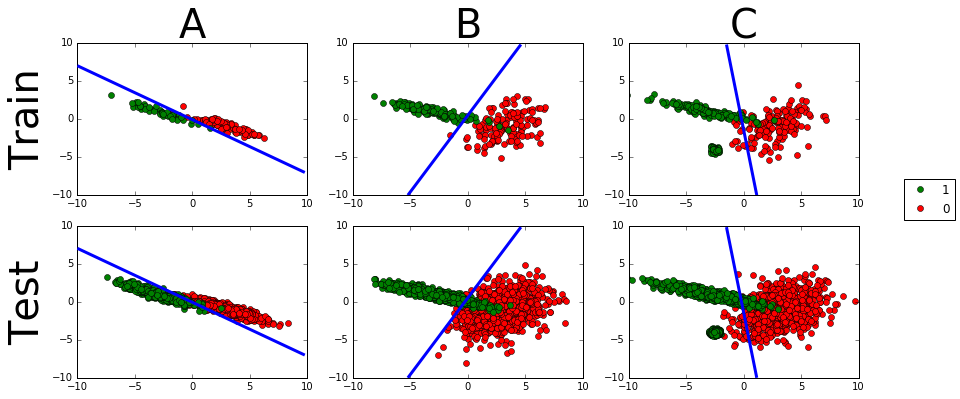
\includegraphics[scale=0.45]{LDA}
    \label{fig:LDA}
    \caption{LDA results}
    \caption*{Les graphes de cette figure représentent les vrai valeurs de y les 1 en vert et 0 en rouge. La ligne bleu déterminée par les données de training de chaque sous ensemble est tracée également sur le graphe du test correspondant. Elle représente l'ensemble des points ou le critère ne sait quelle valeur attribuer a y.}
\end{figure}
\end{enumerate}

\item \textbf{Régression logistique}\\
En reprenant les calculs fait en cours on obtient la formule itérative pour $\omega$:
\begin{align*}
    \omega^{(t+1)} = w^{(t)} + (X^{T}D_{\eta^{(t)}}X)X^{T}(y-\eta^{(t)})
\end{align*}
Néanmoins cette méthode laisse $\omega$ prendre des valeurs assez élevées. Pour palier à ce problème, on ajoute un terme de pénalisation dans la log vraisemblance ($-\frac{\lambda}{2}\lVert\omega\rVert$) cela donne la relation suivante: 
\begin{align*}
    \omega^{(t+1)} = w^{(t)} + (X^{T}D_{\eta^{(t)}}X - \lambda I)(X^{T}(y-\eta^{(t)})-\lambda\omega^{(t)})
\end{align*}
En appliquant cette méthode de descente, on obtient numériquement :
\begin{table}[h!]
    \centering
\begin{tabular}{||c c c||} 
 \hline
 & $\omega$ & $b$\\ 
 [0.5ex] 
 \hline\hline
 A & \begin{pmatrix}
     -8.33972193 \\
    -13.57796665
  \end{pmatrix} & -1.49528825 \\
 \hline
 B & \begin{pmatrix}
    -1.7036036 \\
    1.02265864
  \end{pmatrix} & 1.34676814 \\
 \hline
 C & \begin{pmatrix}
    -2.20181115 \\
    0.70815684
  \end{pmatrix} & 0.95742125 \\
 \hline
\end{tabular}
    \caption{Linear regression learnt parameters}
    \label{tab:lin-reg}
\end{table}
\begin{figure}[h!]
    \centering
    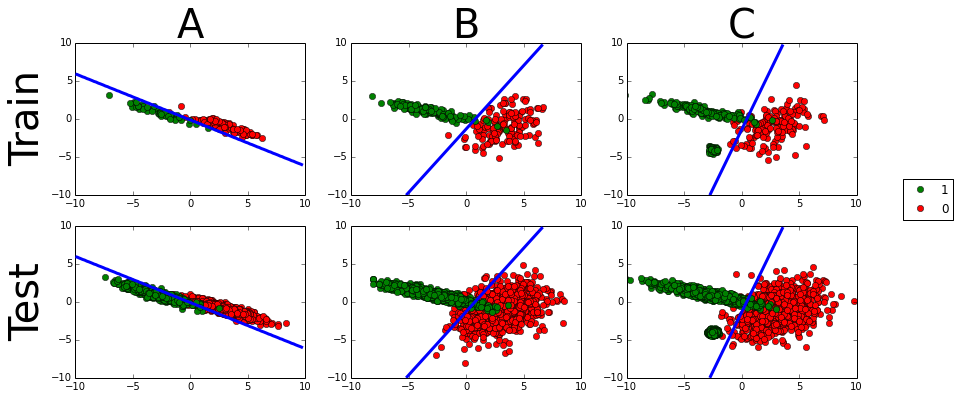
\includegraphics[scale=0.45]{logistic.png}
    \label{fig:reglin}
    \caption{Logistic regression results}
    \caption*{Les graphes de cette figure représentent les vrai valeurs de y les 1 en vert et 0 en rouge. La ligne bleu déterminée par les données de training de chaque sous ensemble est tracée également sur le graphe du test correspondant. Elle représente l'ensemble des points ou le critère ne sait quelle valeur attribuer a y.}
\end{figure}
\newpage
\item \textbf{Régression linéaire}\\
\begin{enumerate}
\item En reprenant le cours sur la régression linéaire dans le cas $b = 0$, l'objectif est de résoudre la "normal equation" : \begin{align*}
X^{T}X\omega-X^{T}y=0
\end{align*}

Ainsi, si $X^{T}X$ est inversible, on obtient :
\begin{align*}
\Aboxed{\widehat{\omega}^{MLE} = (X^{T}X)^{-1}X^{T}y}
\end{align*}

\item 
Pour l'implémentions, on souhaite un $b \neq 0$, pour ce faire on l'inclut dans $\omega$ comme ceci.
\begin{align*}
    Y|X &\sim \mathcal{N}(\omega^{T}X+b, \sigma^2) \\Y&=\omega^{T}X+b+\epsilon \qquad \textrm{avec} \qquad \epsilon \sim \mathcal{N}(0,\sigma^2)
    \\Y&=\widetilde{\omega}^T \begin{pmatrix}
    x \\
    1
  \end{pmatrix} + \epsilon
\end{align*}
On s'est alors ramené a un cas ou le $\widehat{b} = 0$, on peut donc appliquer la formule, puis on extrait la dernière coordonné de $\widetilde{\omega}$ pour avoir les $\omega$ et $b$ cherché. Numériquement, on obtient :
%TABLE DES PARAMETRES
\begin{table}[h!]
    \centering
\begin{tabular}{||c c c||} 
 \hline
 & $\omega$ & $b$\\ 
 [0.5ex] 
 \hline\hline
 A & \begin{pmatrix}
    -0.2640 \\
    -0.3725
  \end{pmatrix} & 0.4922 \\
 \hline
 B & \begin{pmatrix}
    -0.1042 \\
    0.0517
  \end{pmatrix} & 0.5001 \\
 \hline
 C & \begin{pmatrix}
    -0.1276 \\
    -0.0170
  \end{pmatrix} & 0.5083 \\
 \hline
\end{tabular}
    \caption{Linear regression learnt parameters}
    \label{tab:lin-reg}
\end{table}

On a trouver $\omega$ et $b$ pour que $y \simeq \omega^{T}x +b$, donc pour trouver $p(y=1|x_0)=0.5$ on évalue $\simeq \omega^{T}x_0 +b$ et on applique une stratégie de seuil. Si cette valeur est plus grande que 0.5 on attribue a y la valeur 1 sinon 0. On obtient les graphiques des données de train et de test, suivant :
\begin{figure}[h!]
    \centering
    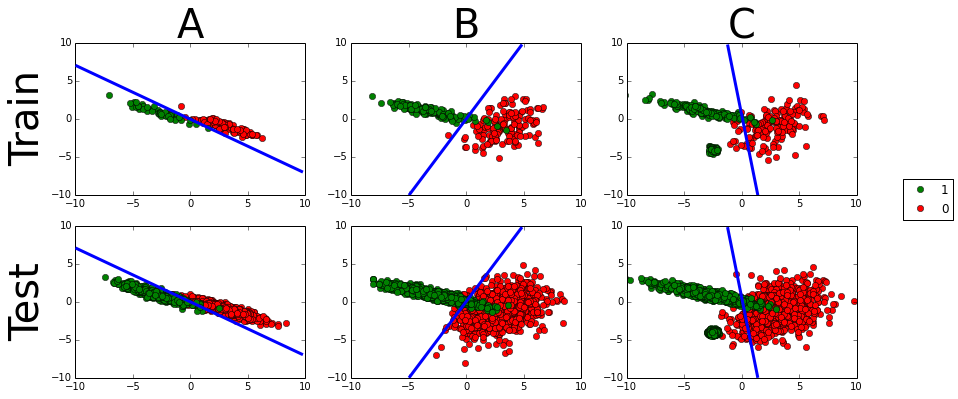
\includegraphics[scale=0.45]{lineaire}
    \label{fig:reglin}
    \caption{Linear regression results}
    \caption*{Les graphes de cette figure représentent les vrai valeurs de y les 1 en vert et 0 en rouge. La ligne bleu déterminée par les données de training de chaque sous ensemble est tracée également sur le graphe du test correspondant. Elle représente l'ensemble des points ou le critère ne sait quelle valeur attribuer a y.}
\end{figure}
\end{enumerate}


\item \textbf{Commentaires et interprétations}\\
\begin{enumerate}
\item Calculons l'erreur de misclassification, i.e la fraction de données mal classifiées pour les données de train et de test : 

%TABLE DES PARAMETRES
\begin{center}
\begin{tabular}{||c c c c c c c||} 
 \hline
 & A_Train & A_Test & B_Train & B_Test & C_Train& C_Test\\ 
 [0.5ex] 
 \hline\hline
 LDA & 1.33\% & 2.00\% & 3.0\% & 4.15\% & 5.5\% & 4.23\% \\
 \hline
 Regression logistique & 0.67\% & 2.53\% & 2.0\% & 4.3\% & 4.0\% & 2.27\% \\
 \hline
 Regression linéaire & 1.33\% & 2.07\% & 3.0\% & 4.15\% & 5.5\% & 4.23\% \\
 \hline
\end{tabular}
\end{center}

\item Les trois méthodes présentées sont des méthodes permettant de faire de la classification avec un critère linéaire. Cela marche bien lorsque l'on a des données qui peuvent être séparé linéairement. On observe cela car ces méthodes performent mieux sur le dataset A que sur le B et le C.\\
Remarquons que l' erreur de misclassification dans le Dataset C est plus importante pour le set de Train que pour celui de Test ce qui est surprenant à premier abord. Cela nous assure au moins qu'on "overfit" pas. Quand on regarde la forme de nos data pour ce Dataset , on remarque que les deux classes sont assez melangé sur une partie et de plus il y a groupement de points, séparés des autres, représentés par les y=1 (en vert), ce qui rend les méthodes de séparation linéaire peu performantes (les erreurs de misclassification pour le dataset C sont les plus élevées).\\
\\
Le fait d'utiliser la régression linéaire pour un problème de classification binaire est assez inintuitif car on modélise notre variable discrète par une variable continue puis on applique un seuil. Néanmoins, elle fournit des résultats extrêmement similaires à la LDA. On peut comprendre cela dataset par dataset:
\begin{description}
  \item[$\bullet$ ] Le A est linéairement séparable et semble vérifier les hypothèse de la LDA
  \item[$\bullet$] Pour les deux autres datasets, ces hypothèses semblent être invalidés
\end{description}

\\
\\\textbf{La régression logistique est celle qui performe globalement le mieux}. Les hypothèses qu'elle suppose sur les données sont moins strictes que les autres méthode et c'est pourquoi elle a de meilleur résultats.
\end{enumerate}
\\
\\
\\ \item \textbf{QDA model}\\

\begin{enumerate}

\item 
Renomons le parametre $\pi$ en $\theta$ pour ne pas qu'il y ait de confusion avec le nombre $\pi$ apparaissant dans la densité de la loi normale. On a donc le modèle suivant:
\begin{align*}
    Y \sim Bernoulli(\theta), \quad X|\{Y=i\} \sim \mathcal{N}(\mu_i,\Sigma_i)
\end{align*}
En procédant exactement comme pour la question 2 sur la LDA, la log vraisemblance s'écrit :
\begin{multline*}
l((\theta,\mu_0,\mu_1,\Sigma_0,\Sigma_1)) =\sum_{n=1}^{N}(y^{(n)}\log(\theta)\ +\  (1-y^{(n)})\log(1-\theta)\ -\ \frac{1}{2}(1-y^{(n)})\log(|\textrm{det}(\Sigma_0)|)\\ -\ \frac{1}{2}y^{(n)}\log(|\textrm{det}(\Sigma_1)|)\\ +\  \bigg((1-y^{(n)})(-\frac{1}{2}((x^{(n)} - \mu_0)^{T}  \Sigma_0^{-1}(x^{(n)} - \mu_0)))\bigg)\\ +\  \bigg(y^{(n)}(-\frac{1}{2}((x^{(n)} - \mu_1)^{T} \Sigma_1^{-1}(x^{(n)} - \mu_1)))\bigg) + cste)\\
\end{multline*}

Ainsi, en dérivant $l((\theta,\mu_0,\mu_1,\Sigma_0,\Sigma_1))$ par rapport à $\theta,\mu_0,\mu_1,\Sigma_0,\Sigma_1$ et en annulant les dérivées, on trouve :
\[\boxed{
\begin{align*} 
\widehat{\theta}^{MLE}&=\frac{\sum_{n=1}^{N}{y^{(n)}}}{N}\\
\widehat{\mu_1}^{MLE}&=\frac{\sum_{n=1}^{N}y^{(n)}x^{(n)}}{\sum_{n=1}^{N}y^{(n)}}
\end{align*}
}\]
\begin{align*} 
\widehat{\mu_0}^{MLE}=\frac{\sum_{n=1}^{N}(1-y^{(n)})x^{(n)}}{\sum_{n=1}^{N}(1-y^{(n)})}
\end{align*}

En raisonnant de manière similaire que pour la LDA, la dérivée de la fonction de log vraisemblance par rapport à $\Sigma_0$ et $\Sigma_1$ donne:
\begin{align*}
\nabla_{\Sigma_0}(l)=\frac{1}{2}\sum_{n=1}^{N}
(1-y^{(n)})\Sigma_0-\frac{1}{2}\sum_{n=1}^{N}
(1-y^{(n)})(x^{(n)}- \mu_0)^{T}(x^{(n)} -\mu_0)\\
\nabla_{\Sigma_1}(l)=\frac{1}{2}\sum_{n=1}^{N}
y^{(n)}\Sigma_1-\frac{1}{2}\sum_{n=1}^{N}
y^{(n)}(x^{(n)}- \mu_1)^{T}(x^{(n)} -\mu_1)
\end{align*}

\\En annulant les dérivées, on trouve les expressions de $\widehat{\Sigma_0}^{MLE}$ et $\widehat{\Sigma_1}^{MLE}$:
\[
\boxed{
\begin{align*}
\widehat{\Sigma_0}^{MLE}&=\frac{\sum_{n=1}^{N}(1-y^{(n)})(x^{(n)}- \mu_0)^{T}(x^{(n)} -\mu_0)}{\sum_{n=1}^{N}(1-y^{(n)})}\\
\widehat{\Sigma_1}^{MLE}&=\frac{\sum_{n=1}^{N}y^{(n)}(x^{(n)}- \mu_1)^{T}(x^{(n)} -\mu_1)}{\sum_{n=1}^{N}y^{(n)}}
\end{align*}
}
\]

L'implémentation des estimateurs du maximum de vraisemblance donnent les résultats numériques suivants pour A, B et C:

%TABLE DES PARAMETRES
\begin{table}[h!]

\resizebox{\textwidth}{!}{\begin{tabular}{||c c c c c c c c c||} 
 \hline
 & $\theta$ & $\mu_0$ & $\mu_1$ & $\Sigma_0$ & $\Sigma_1$ & c & d & M \\ 
 [0.5ex] 
 \hline\hline
 A & 0.3333 & \begin{pmatrix}
    2.8997 \\
    -0.8938
  \end{pmatrix} & \begin{pmatrix}
    -2.6923 \\
    0.8660
  \end{pmatrix} & \begin{pmatrix}
    2.3106 & -1.0474 \\
    -1.0474 & 0.5757
  \end{pmatrix} & \begin{pmatrix}
    2.7044 & -1.3008 \\
    -1.3008 & 0.6896
  \end{pmatrix} & \begin{pmatrix}
     -7.3652 \\
    -10.8733
  \end{pmatrix} & -0.6262 & \begin{pmatrix}
    -1.5174 & -3.0272 \\
    -3.0272 & -5.7233
  \end{pmatrix} \\
 \hline
 B & 0.5 & \begin{pmatrix}
    3.3406 \\
    -0.8354
  \end{pmatrix} & \begin{pmatrix}
    -3.2167 \\
   1.0830
  \end{pmatrix} & \begin{pmatrix}
    2.5388 & 1.0642 \\
    1.0642 & 2.9600
  \end{pmatrix} & \begin{pmatrix}
    4.1536 & -1.3345 \\
    -1.3345 & 0.5160
  \end{pmatrix} & \begin{pmatrix}
    -2.2806\\
    1.4570
  \end{pmatrix} & 3.3665 & \begin{pmatrix}
    -0.9596 & -3.8476 \\
    -3.8476 & -11.0586
  \end{pmatrix} \\
 \hline
 C & 0.625 & \begin{pmatrix}
    2.7930 \\
   -0.8383
  \end{pmatrix} & \begin{pmatrix}
    -2.9423 \\
   -0.9578
  \end{pmatrix} & \begin{pmatrix}
    2.8991 & 1.2458 \\
    1.2458 & 2.9247
  \end{pmatrix} & \begin{pmatrix}
    2.8691 & -1.7619 \\
    -1.7619 & 6.5643
  \end{pmatrix} & \begin{pmatrix}
    -2.6652 \\
    0.3488
  \end{pmatrix} & 0.1100 & \begin{pmatrix}
    0.0048 & -0.2918 \\
    -0.2918 & 0.2361
  \end{pmatrix} \\
 \hline
\end{tabular}}
    \caption{QDA learnt parameters}
    \label{tab:QDA}
\end{table}

\\
\\
\item En ce qui concerne l'expression de la probabilité conditionnelle $p(y=1|x)$, par un calcul similaire à la question 2 sur la LDA, on a :
\begin{align*} 
p(y=1|x)&=\frac{p(x|y=1)p(y=1)}{p(x|y=0)p(y=0) + p(x|y=1)p(y=1)} \\
\\&=\frac{\theta N(x|\mu_1,\Sigma_1)}{(1-\theta)N(x|\mu_0,\Sigma_0) + \theta N(x|\mu_1,\Sigma_1)}\\
\\&=\frac{1}{1+\frac{1-\theta}{\theta}\frac{N(x|\mu_0,\Sigma_0)}{N(x|\mu_1,\Sigma_1)}}\\
\\&=\frac{1}{1+\frac{1-\theta}{\theta}\frac{\sqrt{|\textrm{det}(\Sigma_1)}|}{\sqrt{|\textrm{det}(\Sigma_0)}|}\exp(\frac{1}{2}((x^{(n)} - \mu_1)^{T} \Sigma_1^{-1}(x^{(n)} - \mu_1)-(x^{(n)} - \mu_0)^{T} \Sigma_0^{-1}(x^{(n)} - \mu_0)))}
%\\
%\\&=\frac{1}{1+\exp(-fonction \ linéaire)}
\end{align*}

Ainsi, on effectue les transformations suivantes pour faire apparaitre la fonction sigmoide : 
\begin{align*} 
p(y=1|x)&=\frac{1}{1+\frac{1-\theta}{\theta}\frac{\sqrt{|\textrm{det}(\Sigma_1)}|}{\sqrt{|\textrm{det}(\Sigma_0)}|}\exp(-[\frac{1}{2}x^{(n)}(\Sigma_0^{-1}-\Sigma_1^{-1})x^{(n)}+(\mu_1^{T}\Sigma_1^{-1}-\mu_0^{T}\Sigma_0^{-1})x^{(n)}+(\frac{1}{2}(\mu_0^{T}\Sigma_0^{-1}\mu_0-\mu_1^{T}\Sigma_1^{-1}\mu_1))])}
\\&= \sigma(\frac{1}{2}x^{(n)}^TMx^{(n)}+c^Tx^{(n)}+d)
\end{align*}

avec $\sigma$ la fonction sigmoide, et :
\begin{align*} 
M=\Sigma_0^{-1}-\Sigma_1^{-1}
\end{align*}

\begin{align*} 
c=\mu_1^{T}\Sigma_1^{-1}-\mu_0^{T}\Sigma_0^{-1} \qquad \qquad d=\log(\frac{\theta}{1-\theta})+\frac{1}{2}\log(\frac{|\textrm{det}(\Sigma_0)|}{|\textrm{det}(\Sigma_1)|})+ \frac{1}{2}(\mu_0^{T}\Sigma_0^{-1}\mu_0-\mu_1^{T}\Sigma_1^{-1}\mu_1)
\end{align*}
La figure \ref{fig:QDA} est la représentation graphique des données de train et de test. Dans ce cas, la frontière de décision définie par $p(y=1|x)=0.5$ est une elliptique car c'est la solution d'une quadratique~=~0:
\begin{figure}[h!]
    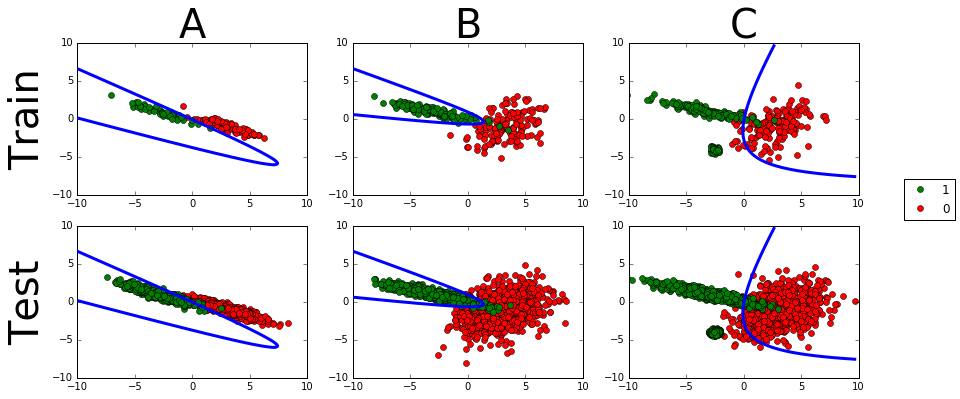
\includegraphics[scale=0.45]{QDA}
    \caption{QDA results}
    \caption*{Les graphes de cette figure représentent les vrais valeurs de y les 1 en vert et 0 en rouge. La ligne bleu déterminée par les données de training de chaque sous ensemble est tracée également sur le graphe du test correspondant. Elle représente l'ensemble des points ou le critère ne sait quelle valeur attribuer a y.\label{fig:QDA}}
\end{figure}

\\
\\
\item
Calculons l'erreur de misclassification pour les données de train et de test :
%TABLE DES PARAMETRES
\begin{center}
\begin{tabular}{||c c c c c c c||} 
 \hline
 & A_Train & A_Test & B_Train & B_Test & C_Train& C_Test\\ 
 [0.5ex] 
 \hline\hline
 LDA & 1.33\% & 2.00\% & 3.0\% & 4.15\% & 5.5\% & 4.23\% \\
 \hline
 Regression logistique & 0.67\% & 2.53\% & 2.0\% & 4.3\% & 4.0\% & 2.27\% \\
 \hline
 Regression linéaire & 1.33\% & 2.07\% & 3.0\% & 4.15\% & 5.5\% & 4.23\% \\
 \hline
 QDA & 0.67\% & 2.00\% & 1.33\% & 2.0\% & 5.25\% & 3.83\% \\
 \hline
\end{tabular}
\end{center}

\\
\\
\\
\item

Pour le dataset A, on voit que la LDA fait aussi bien que les premières méthode. En effet il semble que l'hypothèse que $\Sigma_1 = \Sigma_2$ soit bonne donc la LDA est suffisante.

\\Pour le dataset B, la frontière de décision définie par $p(y=1|x)=0.5$ est une conique ce qui garantit que la QDA - qui est un modèle plus complexe que la LDA - performe beaucoup mieux que tous les autres modèles (l'erreur de misclassification est la plus basse). La QDA semble être le modèle adapté pour la séparation des données de ce dataset.


\\Pour le dataset C, on note une amélioration de l'erreur, la QDA permet de mieux séparer les points proche de la zone ou les deux classes se chevauchent. Mais on arrive aux mêmes conclusions que précédemment, à savoir que le le groupement de points vert séparés des autres nous laisse penser que l'hypothèse que $X|Y$ suit une loi normale est fausse. C'est pourquoi l'erreur ne décroît pas autant que sur le dataset B. On remarque d'ailleurs que a cause du groupement un peu a l'écart des point 1, dans le cas C la décision essaye d'exclure les point 0, alors que dans le cas B ou il n'y a pas cette singularité la courbe essaye d'inclure les 1.

\end{enumerate}
\end{enumerate}
\end{document}
